Para el desarrollo de la aplicación, utilizaremos una metodología similar a la empleada en el desarrollo de videojuegos tradicional. Por lo tanto, explicaremos las diferentes fases de este proceso, definiendo los objetivos a alcanzar en cada una de ellas.

\section{Metodología}

El proyecto ARTEMIS tiene como objetivo desarrollar una aplicación que pueda ser utilizada como herramienta complementaria en sesiones de musicoterapia. El enfoque de la investigación reside en el desarrollo iterativo de videojuegos serios que se fundamenten en evaluaciones empíricas de su efectividad. Esto significa que se aplicará la metodología de desarrollo de videojuegos serios, la cual es muy similar al desarrollo de videojuegos convencionales. Describiremos las principales fases del desarrollo de la aplicación para llegar a una versión final.

\subsection{Investigación inicial y revisión de literatura}

El objetivo principal de esta fase es recopilar y analizar estudios previos sobre las líneas de investigación relevantes para el desarrollo de esta aplicación. Esta investigación finalizará en el análisis del uso de videojuegos serios en terapias para la ansiedad. Esta etapa es esencial para establecer una base teórica sólida y comprender el estado actual de la investigación en este campo. Además, permitirá identificar brechas en estas áreas donde la nueva investigación pueda aportar contribuciones.

Para lograr esto, se lleva a cabo una revisión sistemática de la literatura que implica recopilar, evaluar y sintetizar información relevante en los campos específicos de la investigación. Esta literatura está conformada por bibliografía de bases de datos como Google Scholar, PubMed o Dialnet. Aunque esta fase se ha realizado antes del desarrollo, en el capítulo \ref{chapter:state}, es relevante incluirla en la metodología. Esto se debe a que es el paso inicial fundamental para fundamentar las decisiones que se van a tomar en las siguientes fases del desarrollo.

\subsection{Conceptualización y diseño}

El objetivo de esta fase es definir los elementos clave para el diseño y funcionalidad de la aplicación. Esto incluye la identificación de las mecánicas de juego que se utilizarán, y la creación de nuevas mecánicas si fuera necesario. Es importante en esta fase justificar las decisiones de diseño tomadas, manteniendo siempre la alineación con las bases terapéuticas de las investigaciones de la fase anterior. 

Para diseñar las mecánicas del juego, es esencial considerar los elementos de diseño de videojuegos serios, los diferentes tipos de ansiedad junto con sus respectivos tratamientos, y las modalidades de musicoterapia. El autor de este trabajo aportará ideas sobre posibles mecánicas, las cuales se complementarán con sesiones de brainstorming entre los miembros del proyecto ARTEMIS y la tutora de este TFG. De esta forma, se conseguirá conceptualizar diversas mecánicas centradas en estos aspectos, que podrán ser desarrolladas una vez se cambie a la siguiente fase.

\subsection{Desarrollo iterativo}

El desarrollo iterativo es un enfoque importante en la creación de videojuegos. Permite mejorar el producto en desarrollo a través de ciclos repetidos de diseño, prueba y pulido. Este proceso es esencial para garantizar que el videojuego sea no solo funcional, sino también eficaz a nivel terapéutico. Es vital recoger feedback sobre los aspectos positivos y negativos de las distintas iteraciones para lograr un resultado final óptimo tras las necesarias revisiones.

El objetivo de esta etapa será crear prototipos del videojuego en cuestión y perfeccionarlos continuamente hasta obtener un resultado que cumpla con los objetivos terapéuticos y ofrezca una experiencia de usuario adaptada al contexto. Este proceso se basa en recibir feedback de los miembros del equipo y las directivas, así como tener en cuenta la opinión de equipos externos de psicología y música.

El prototipado será de gran importancia para conseguir un resultado mecánico atractiva y que funcione alrededor de los conceptos terapéuticos. Una vez se haya alcanzado un prototipo acorde a estos principios, se desarrollará una versión más pulida y con elementos de juego finales como arte y audio.

Para un correcto cumplimiento de esta fase, utilizaremos una metodología ágil para iterar sobre el desarrollo. Scrum, como metodología, divide el desarrollo en sprints cortos y manejables, permitiendo ajustes continuos basados en el feedback rápido que proporcionan este tipo de sistemas. Además, al final de cada sprint, se pueden realizar retrospectivas para evaluar el progreso del proyecto y proponer mejoras estructurales para los próximos sprints.

\subsection{Mejora continua}

Esta fase realmente no pertenece al desarrollo, sin embargo, y aunque se mencionará en profundidad en las conclusiones de este TFG, al ser un proyecto de investigación vivo, incluso tras la finalización de este trabajo, está en constante cambio. Está planteado

\newpage

\section{Tecnologías empleadas}

Las tecnologías utilizadas para el desarrollo de la aplicación se pueden clasificar según su uso. Debido a que el formato propuesto para el desarrollo es similar al de un videojuego, donde la interacción es esencial para su uso correcto y óptimo, se ha seleccionado software adecuado para el producto realizado. A continuación, se explicará detalladamente el uso de las diferentes tecnologías y las razones detrás de la elección de cada una específicamente.

\subsection{Unity}

Un motor de videojuegos, del inglés game engine, es un entorno que proporciona un conjunto de herramientas reutilizables que facilitan la creación de videojuegos a los desarrolladores. Estos se pueden dividir en el motor gráfico, responsable del aspecto visual, y el motor físico, encargado de dotar al motor de leyes físicas como la gravedad, la masa o las fuerzas. Cada motor de videojuegos tiene sus propios usos y limitaciones. Por lo tanto, la elección del motor a utilizar es de gran importancia antes de iniciar el desarrollo. Existen motores más especializados en el desarrollo 3D como \textit{Unreal Engine} (\cite{UE:1998}), mientras que otros están centrados en gráficos 2D, como \textit{Game Maker Studio} (\cite{GMS:1999}) y \textit{RPG Maker} (\cite{RPGM:1992}). \textit{Unity} (\cite{UNITY:2005}) y \textit{Godot Engine} (\cite{GODOT:2001}) son híbridos que permiten el desarrollo en ambas dimensiones.

Unity, junto con Unreal Engine y recientemente Godot Engine, es uno de los motores de videojuegos más populares en la industria. Aunque Unreal Engine es valorado como posiblemente el mejor motor de videojuegos de la actualidad, su uso está limitado a circunstancias muy específicas: videojuegos 3D para consolas de última generación. Sin embargo, Unity, aunque no ofrece la potencia gráfica de Unreal Engine, es mucho más versátil y se puede utilizar en una amplia variedad de circunstancias. Esto permite que el rango de plataformas para las que se puede desarrollar con este motor aumente, convirtiéndolo en una opción más segura para enfocarse en el desarrollo multiplataforma.

\begin{figure}[h!]
	\centering
	\subfigure[Unity.]{
\includegraphics[width=0.2\textwidth]{./Figuras/Aspectos/UnityLogo}\label{fig:UnityLogo}}
	\hfil
	\subfigure[Unreal Engine.]{
\includegraphics[width=0.2\textwidth]{./Figuras/Aspectos/UnrealLogo.png}\label{fig:UnrealLogo}}
	\hfil
	\subfigure[Godot Engine.]{
\includegraphics[width=0.2\textwidth]{./Figuras/Aspectos/GodotLogo.png}\label{fig:GodotLogo}}
	\caption[Logotipos de motores Unity, Unreal Engine y Godot Engine.]{Logotipos de los motores de videojuegos mencionados en el párrafo anterior.}
	\label{fig:GameEngineLogos}
\end{figure}

Hemos seleccionado Unity para nuestro caso específico por diversas razones, dado que la aplicación se desarrolla completamente en 2D y nuestra plataforma objetivo son los dispositivos móviles, en particular las tabletas. Unity domina el 50\% del desarrollo de videojuegos para móviles, consolas y PC, con un 71\% de los 1000 mejores juegos móviles creados en Unity (\cite{PLARIUM:2024}).

El motor gráfico 2D de Unity ofrece diversas herramientas útiles para el desarrollo, como el Sprite Editor. Además, Unity tiene una sólida integración de físicas 2D que permite simular colisiones, gravedad y otros elementos físicos. Su interfaz es intuitiva y fácil de usar, como se muestra en la \autoref{fig:UnityUI}, facilitando la creación rápida de videojuegos.

\begin{figure}[h!]
	\centering
	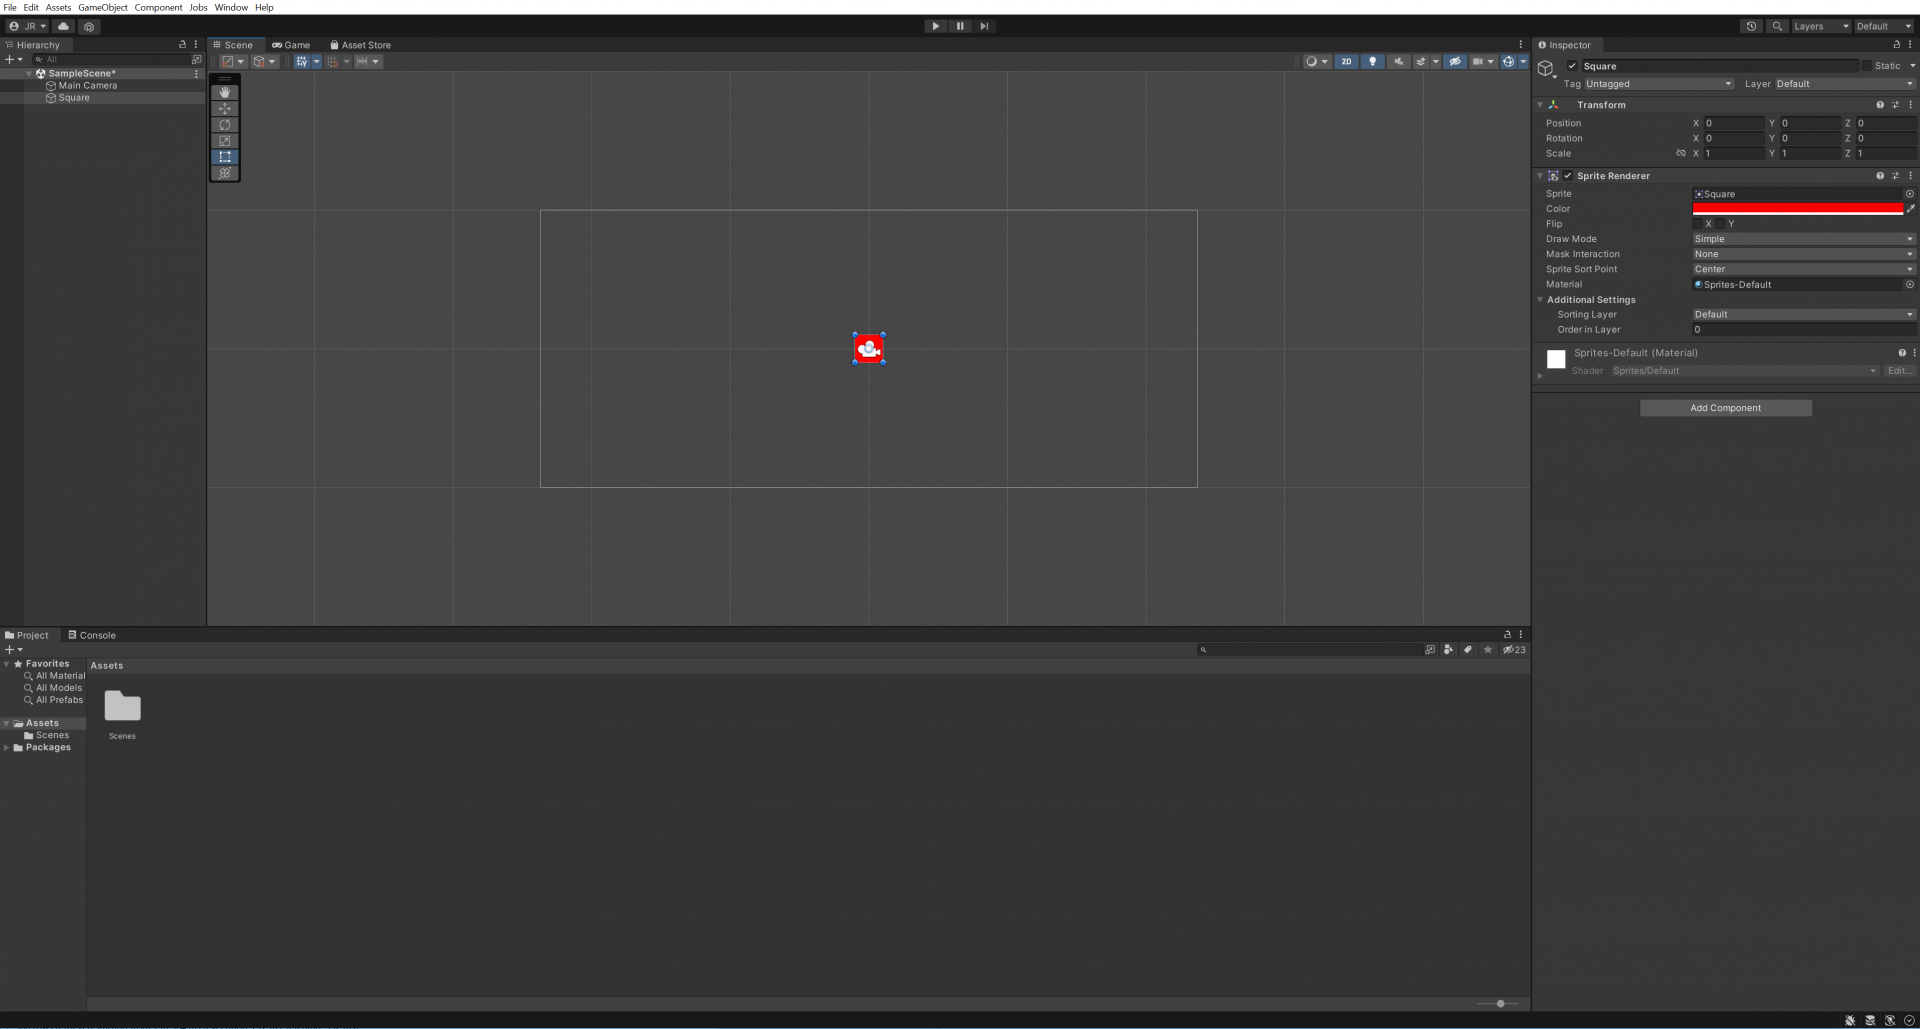
\includegraphics[width=0.7\linewidth]{./Figuras/Aspectos/UnityUI.png}
	\caption{Interfaz de usuario de la plantilla 2D de Unity.}
	\label{fig:UnityUI}
	\vspace{-30pt}
\end{figure}

\begin{center}
	\textbf{Fuente:} Captura realizada por el autor del TFG.
\end{center}

La capacidad de arrastrar y soltar objetos en el editor de Unity simplifica significativamente el proceso de diseño, permitiendo a los desarrolladores centrarse en la creatividad y la jugabilidad en lugar de en aspectos técnicos complejos. Además, Unity cuenta con una comunidad amplia y activa que ofrece acceso a foros, tutoriales, cursos en línea y documentación extensa. Esta comunidad es un recurso invaluable para obtener soporte y encontrar soluciones a problemas comunes, aprender técnicas nuevas y compartir experiencias.

La Asset Store de Unity ofrece una gama variada de recursos como sprites, animaciones, scripts y plugins, que pueden agilizar el desarrollo. Estos recursos preconstruidos permiten a los desarrolladores integrar rápidamente elementos visuales y funcionales complejos sin la necesidad de crearlos desde cero, ahorrando tiempo y esfuerzo.

Todos estos factores, sumados a que Unity es el motor en el que más experiencia tenemos, fueron decisivos para seleccionarlo como el motor de desarrollo para ARTEMIS. La versión seleccionada es la 2021.3.31f, que fue la última versión de soporte a largo plazo (LTS) disponible en el momento en que se inició el proyecto.

\subsection{Visual Studio 2022 (C\#)}

Visual Studio es un entorno de desarrollo integrado (IDE) y editor de código, creado por Microsoft en 1997. Este editor es compatible con numerosos lenguajes de programación, como C++, Visual Basic .NET, Fortran, J\# y, más relevante para nuestro desarrollo, C\#. Su versión 2022 es la última versión disponible actualmente, y ha incorporado mejoras de rendimiento y nuevas funciones de accesibilidad para el usuario. Visual Studio, junto con Visual Studio Code y JetBrains Rider, forma el conjunto de editores de código con la mejor integración con Unity.

\subsection{FMOD}

FMOD Studio es un middleware\footnote{Un middleware, en términos de informática, es un software que facilita la comunicación entre las distintas aplicaciones y el sistema operativo. Además, proporciona funcionalidades inteligentes que permiten una innovación más rápida y un desarrollo eficiente. En el desarrollo de videojuegos, el middleware es un software que facilita la implementación de funcionalidades específicas dentro del motor.} de audio para videojuegos. Fue desarrollado y lanzado por Fireflight Technologies en 1995. Este motor de música y efectos de sonido se asemeja a un DAW tradicional, como se puede observar en la \autoref{fig:FMODUI}. FMOD Studio pertenece a la misma familia que el middleware Audiokinetic Wwise. Ambos proveen herramientas para la sonorización de videojuegos que facilitan la implementación de audio. Sin embargo, se ha decidido utilizar FMOD Studio debido a la mayor familiaridad con este software.

\begin{figure}[h!]
	\centering
	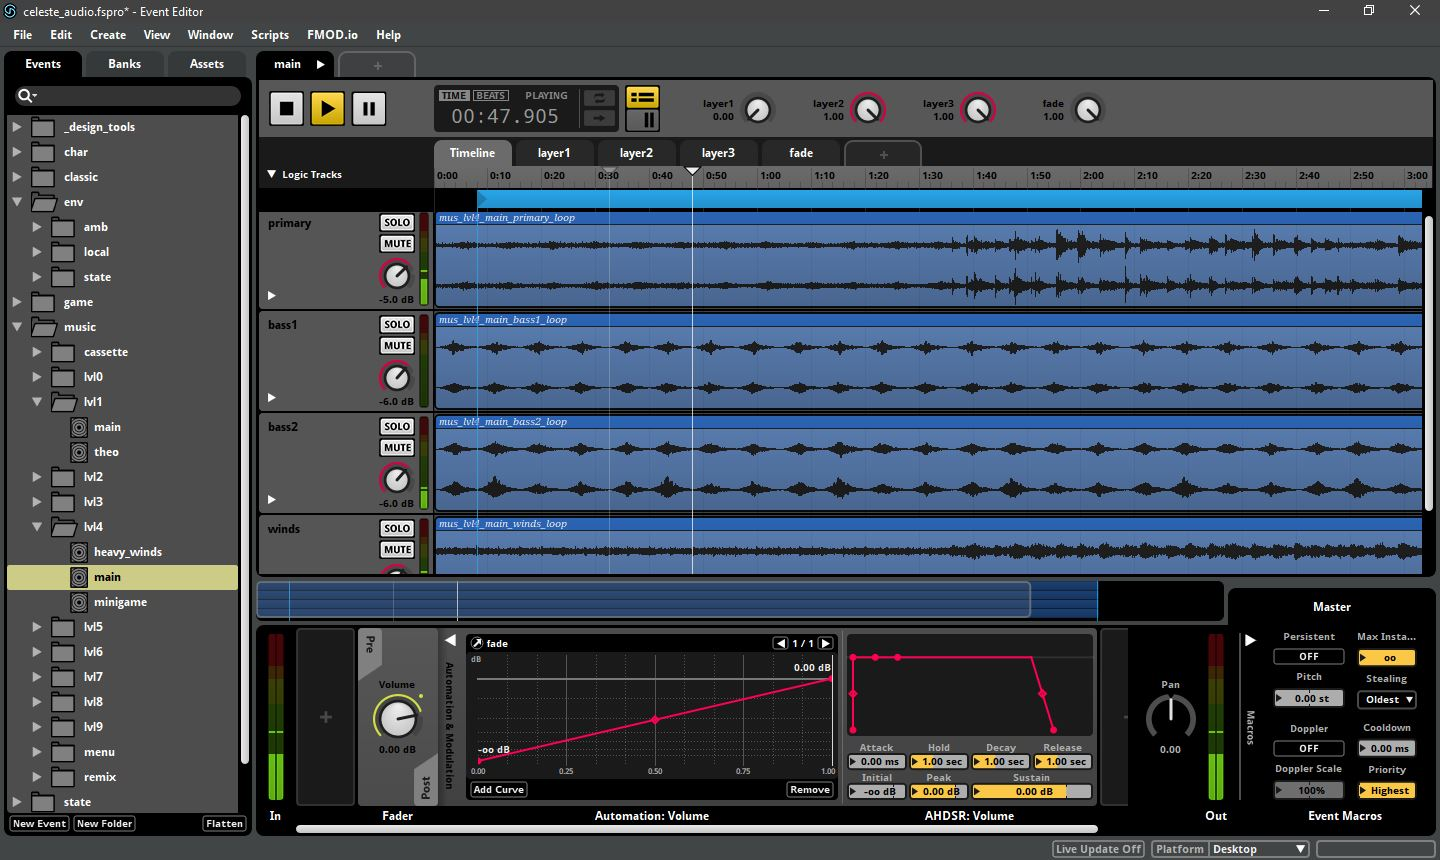
\includegraphics[width=0.9\linewidth]{./Figuras/Aspectos/FMODStudio.jpg}
	\caption{Interfaz de usuario de FMOD Studio.}
	\label{fig:FMODUI}
	\vspace{-30pt}
\end{figure}

\begin{center}
	\textbf{Fuente:} \citeauthor{FMODSTUDIO:2024} (\citeyear{FMODSTUDIO:2024}).
\end{center}

A diferencia del sistema de audio de Unity, que tiene funcionalidades limitadas, FMOD Studio permite gestionar con gran precisión las pistas de audio en eventos, incluso utilizando filtros de diversos tipos si fuera necesario. Desde FMOD Studio, se pueden añadir parámetros asociados a zonas de bucle, compases musicales o pistas, que luego pueden ser modificados desde los propios componentes de Unity o por programación de scripts en función de las necesidades del videojuego que se esté desarrollando.

\subsection{TeXstudio}

TeXstudio es un editor de LaTeX de código abierto lanzado en 2009 que ofrece un soporte moderno para la escritura. Cuenta con funcionalidades como la corrección ortográfica interactiva, el plegado de código y el resaltado de sintaxis. La decisión de utilizar un editor de LaTeX en lugar de editores de texto convencionales, como Word, se basa en la magnitud del documento. LaTeX ofrece citación y referencia automáticas de figuras o tablas, proporcionando estabilidad y sostenibilidad al documento. También permite almacenar toda la bibliografía en una base de datos con toda la información relevante de la cita, incluyendo referencias sobre el autor, fecha, enlaces y otros datos de interés. Los datos se pueden citar manualmente o automáticamente según un sistema de citas específico, en nuestro caso APA 7. Al combinarse con la distribución Miktex, la instalación automática de paquetes y la actualización a las últimas versiones tanto de los paquetes como de TeXstudio, asegura mantener siempre actualizado el software.

\subsection{GitHub}

GitHub es un repositorio que utiliza el control de versiones de Git para alojar proyectos. La utilización de GitHub ha facilitado la colaboración entre los distintos miembros del grupo de investigación, permitiendo a cada uno trabajar en diferentes aspectos del proyecto de forma simultánea. Tiene un sistema de revisión de código, en forma de pull requests\footnote{Un pull request es una solicitud en la que un colaborador solicita al administrador que revise los cambios que ha realizado, antes de fusionarlos con la rama principal del proyecto.}, que asegura que todos los cambios tengan que ser aprobados antes de poder ser integrados en la rama principal del proyecto, añadiendo una capa de protección que otorga seguridad al código. Tiene integración directa con Unity y LaTeX, por lo que ha sido muy útil para permitir el trabajo remoto entre los distintos miembros del grupo de investigación e incluso para trabajar en distintos dispositivos sin necesidad de migrar manualmente el proyecto. El uso del repositorio nos ha brindado una serie de comodidades que, sin su utilización, habrían obstaculizado el progreso eficiente del proyecto, ya sea por las posibles restricciones geográficas del equipo o por el número de miembros que lo conforman.